% SVN info for this file
\svnidlong
{$HeadURL$}
{$LastChangedDate$}
{$LastChangedRevision$}
{$LastChangedBy$}

\chapter{Teoria della misura}
\labelChapter{teoriamisura}

\begin{introduction}
	‘‘Se la tua nuova teoria si può esprimere con grande semplicità, allora esisterà un'eccezione patologica ad esso!''
\begin{flushright}
	\textsc{Adrian Mathesis,} adirato per essere stato bocciato da Riemann.
\end{flushright}
\end{introduction}
\lettrine[findent=1pt, nindent=0pt]{N}{el} corso di \textsc{Analisi Matematica Uno} abbiamo dato la definizione di integrale secondo Riemann per funzioni limitate come generalizzazione del concetto di ‘‘calcolo delle aree''. Per quanto utile e sufficientemente complesso, questo strumento matematico ha tutta una serie di \textit{limiti} e di \textit{stranezze}, tra cui:
\begin{itemize}
	\item Cambiare il valore che una funzione Riemann-integrabile assume in un certo punto può far sì che, se il valore è infinito, la funzione non ammette più integrale - anche se intuitivamente l'area sottesa da un singolo punto è sempre nulla!.
	\item Ci sono funzioni che, pur essendo costanti tranne un numero numerabile di punti, \textit{non} ammettono integrale, mentre le funzioni limitate e continue tranne un numero numerabile di punti sono Riemann integrabili.
	\item Ci sono sequenze di funzioni Riemann-integrabili che convergono a funzioni non integrabili.
	\item L'integrale di Riemann è propriamente integrabile solo in intervalli chiusi (o al più unioni di essi) e, se siamo abbastanza audaci, su intervalli illimitati; all'apparenza si escludono dal concetto di integrazione tutti gli insiemi non riconducibili agli intervalli.
	\item Dato che la definizione si basa sulle partizioni, che necessitano della metrica di $\realset$, non si può applicare l'integrale di Riemann a spazi astratti e funzioni definite su di essi. In particolare, non si possono calcolare per le successioni $f(n)=f_n$, per le quali sembra invece intuitivo supporre che
	\begin{equation*}
		\int f=\sum f_n
	\end{equation*}
	In questo modo si potrebbero applicare i teoremi sugli integrali al mondo delle serie! 
\end{itemize}
\parshape=0
Vogliamo dunque definire un concetto di integrazione più generale dell'integrale di Riemann, ma che sia compatibile con esso e mantenga le sue proprietà ‘‘buone''. Dato che una delle principali limitazioni dell'integrale di Riemann è essere basato sulla \textit{lunghezza} delle partizioni del dominio su cui integriamo, abbiamo necessariamente bisogna prima di generalizzare questo concetto.\\
L'\textbf{integrale di Lebesgue}, così chiamato in onore del suo ideatore Henri \textbf{Lebesgue} (1875-1941), e la \textbf{teoria della misura} cercano di soddisfare proprio queste richieste.\\
In questo capitolo, dopo un excursus storico su come siamo arrivati a questi due concetti, ci dedicheremo completamente alla \textbf{misura}, prima su $\realset$ e $\realset^n$ per poi generalizzarlo sugli spazi cosiddetti \textbf{misurabili}.
\section{Il contesto storico: il problema delle discontinuità nell'integrale definito}
Seppur tecniche per calcolare aree e volumi furono già introdotte dai matematici dell'antica Grecia, fu solo nel tardo XVII secolo che vennero sviluppati i principi dell'integrazione indipendentemente da Isaac Newton (1643-1727) e Gottfried Wilhelm Leibniz (1646-1716), i quali immaginarono l'area sotto una curva come una \textit{somma infinita} di rettangoli di \textit{larghezza infinitesima}.\\
La formalizzazione di questo concetto arrivò nel corso dell'Ottocento grazie a Augustin-Louis \textbf{Cauchy} (1789-1857), che in \textit{Résumé des leçons données à l’École Royale Polytechnique sur le calcul infinitésimal (1823)} definì l'integrale per funzioni continue su un dominio compatto con al più un numero finito di discontinuità.\\
Come ogni matematico che si rispetti, subito dopo aver letto questa definizione quello che fecero gli analisti dell'Ottocento fu chiedersi:
\begin{center}
	\textit{Come allargare la \textbf{classe} delle funzioni che ammettono integrale?}
	\textit{Come posso \textbf{caratterizzare} i \textbf{punti di discontinuità} di una funzione
		integrabile?}\\
\end{center}
Per la seconda domanda ci furono diversi approcci: alcuni ipotizzarono che la \textit{cardinalità} dell'insieme delle discontinuità dovesse essere piccola, altri pensarono che bisognasse passare per proprietà topologiche\footnote{Anche se i primi concetti di Topologia si possono ricondurre al famoso ‘‘Problema dei ponti di Königsberg'' affrontato da Eulero , furono proprio gli analisti ottocenteschi, bramosi di risolvere il problema delle discontinuità dell'integrale, a dare impulso a questa branca della matematica. Per alcuni cenni al mondo della Topologia rimandiamo il lettore curioso a \cite{antucabertolotti:2021manualozzogeometria}.} come densità, ecc...\\
Per la prima, invece, Bernhard \textbf{Riemann} (1826-1866) nella sua \textit{Tesi di abilitazione all'insegnamento (1851-1852)} estese il concetto di integrale alle funzioni limitate e diede una caratterizzazione delle funzioni integrabili (ora dette \textbf{integrabili secondo Riemann}).
\begin{define}[Caratterizzazione degli integrali secondo Riemann]
La funzione $\funz{f}{\left[a,b\right]}{\realset}$ limitata è \textbf{integrabile} (secondo Riemann) se e solo se $\forall \epsilon>0,\ \exists D$ suddivisione di $\left[a,b\right]$ in un numero finito di intervalli $I_1,\ \ldots,\ I_n$ tale per cui
\begin{equation}
	\sum_{i=1}^{n}\left(\sup_{I_i}f-\inf_{I_i}f\right)\mathcal{L}\left(I_i\right)<\epsilon
\end{equation}
\end{define}
Per quanto questo fu un passo avanti, l'integrale di Riemann non era sufficiente a risolvere tutti i problemi sorti: infatti, non tutte le funzioni limitate risultano essere integrabili!\\
Dalla caratterizzazione di Riemann è evidente che affinché una funzione sia integrabile è necessario rendere \textit{piccola} l’\textit{oscillazione} di $f$, ossia
\begin{equation*}
	\sup_{I_i}f-\inf_{I_i}f
\end{equation*}
Dal teorema di \textit{Heine-Cantor} è noto che per le funzioni continue su $\left[a,b\right]$ questa oscillazione è arbitrariamente piccola se l’ampiezza dell’intervallo $I_i$ è
sufficientemente piccola, mentre in generale \textit{non lo è}.
\begin{examplewt}[La funzione di Dirichlet]\label{funzionedirichlet}
	Consideriamo la \textbf{funzione di Dirichlet}\footnote{Peter Gustav Lejeune \textbf{Dirichlet} (1805-1859) fu il primo a studiarne le proprietà.}\index{funzione!di Dirichlet}
	\begin{equation}
		f(x)=
		\begin{cases}
			\begin{array}{ll}
				1&\text{se }x\in\left[0,1\right]\cap\rationalset\\
				0&\text{se }x\in\left[0,1\right]\setminus\rationalset\\
			\end{array}
		\end{cases}
	\end{equation}
Osserviamo come essa \textit{non} è integrabile su $\left[0,1\right]$: poiché $\forall D$ partizione di $\left[0,1\right]$ per densità dei razionali si ha
\begin{equation*}
	\sup_{I_i}f=1\qquad	\inf_{I_i}f=1,\ \forall i=1,\ldots,n
\end{equation*}
Allora
\begin{equation*}
	\sum_{i=1}^{n}\left(\sup_{I_i}f-\inf_{I_i}f\right)\mathcal{L}\left(I_i\right)=\sum_{i=1}^{n}\left(1-0\right)\mathcal{L}\left(I_i\right)=\sum_{i=1}^{n}\mathcal{L}\left(I_i\right)=\mathcal{L}\left(\left[0,1\right]\right)=1,\ \forall D\text{ sudd.}
\end{equation*}
\end{examplewt}
Nonostante il profuso impegno, non si riuscì in alcun modo a collegare la cardinalità o delle proprietà topologiche all'insieme dei punti di discontinuità. Per quasi cinquant'anni l'integrale rimase più o meno nella stessa forma data da Riemann\footnote{Nel 1894 Thomas Joannes \textbf{Stieltjes} (1856-1894) pubblicò una generalizzazione dell'integrale di Riemann che oggi prende il nome di \textbf{integrale di Riemann-Stieltjes}; qui non lo tratteremo, ma è doveroso segnarlo come un importante precursore di quello che sarà l'\textit{integrale di Lebesgue}.} fino al 1902, quando Henri Lebesgue (1875-1941) nella sua tesi di laurea \textit{Intégrale, longueure, aire (1902)} introdusse i concetti di \textbf{misura} $n$-dimensionale e di \textbf{integrale secondo Lebesgue}.\\
L’idea di Lebesgue si basa su una semplice osservazione: per rendere piccola l’oscillazione di $f$ il procedimento \textit{naturale} non è, come fa Riemann, di partizionare in piccoli intervalli il suo \textit{dominio}, bensì di suddividere in intervalli
di ampiezza piccola l’\textbf{immagine} di $f$.\\
\begin{minipage}{0.5\textwidth}
	\begin{center}
		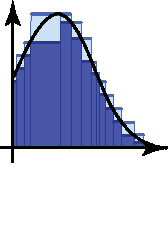
\includegraphics[trim=0cm 0cm 0cm 0cm, clip, scale=1.6]{images/lebesgueriemann1}
	\end{center}
\end{minipage}
\begin{minipage}{0.5\textwidth}
	\begin{center}
		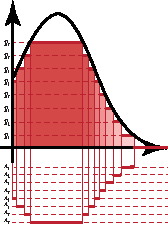
\includegraphics[trim=0cm 0cm 0cm 0cm, clip, scale=1.6]{images/lebesgueriemann2}
	\end{center}
\end{minipage}\\
In \textit{Sur le development de la notion d'intégrale (1926)} Lebesgue ripercorre il procedimento naturale alla base di questa idea fondamentale:
\blockquote{
	‘‘I geometri del diciassettesimo secolo considerano l'integrale di $f(x)$ - la parola \textit{integrale} non era ancora stata inventata, ma non importa - come la somma di un'infinità di indivisibili, ognuno dei quali era l'ordinata, positiva o negativa, di $f(x)$.\\
	Benissimo! Noi abbiamo semplicemente raggruppato insieme gli \textit{indivisibili} di 	grandezza vicina. Abbiamo, come si dice in algebra, riunito termini simili. Si potrebbe dire che, secondo il procedimento di Riemann, si cerca di sommare gli indivisibili prendendoli \textit{nell’ordine nel quale ci sono forniti dalla variazione di $x$}, come un commerciante confusionario che conta monete e biglietti a caso,	nell’ordine in cui gli vengono dati, mentre noi operiamo come un commerciante metodico che dice:
	\begin{center}
		 \begin{tabular}{l}
			«ho $m(G_1)$ monete da $100$, che valgono $100\ m(G_1)$»\\
			«ho $m(G_2)$ monete da $500$, che valgono $500\ m(G_2)$»\\
			«ho $m(G_3)$ biglietti da $1000$, che valgono $1000\ m(G_3)$»\\
			...
		\end{tabular}
	\end{center}
	Tutto insieme ho
	\begin{equation*}
		S=100\ m(G_1) + 500 m(G_2)+ 1000 m(G_3)+\ldots
	\end{equation*}
	I due procedimenti porteranno di certo il commerciante allo stesso risultato perché per quanti soldi abbia c’è solo un numero finito di monete e di biglietti da contare. Ma per noi che dobbiamo sommare un numero infinito di indivisibilità la differenza dei due metodi è \textit{di capitale importanza}.''
}
In altre parole, per calcolare l'integrale (secondo Lebesgue) di una funzione:
\begin{itemize}
	\item Suddividiamo l'immagine in intervalli e per ognuno di essi consideriamo un \textit{peso} dato dall'\textit{estremo inferiore} dei valori assunti dalla funzione nel dato intervallo.
	\item Consideriamo le controimmagini degli intervalli e associamo a ciascuna un valore detto \textbf{misura}.
	\item Calcoliamo un'approssimazione \textit{per difetto} dell'integrale sommando le misure che abbiamo ottenuto - ciascuna moltiplicata per il corrispondente peso.
	\item Più fitta è la partizione iniziale, più accurato sarà il valore dell'integrale.
\end{itemize}
\begin{intuit}
Poiché partizioniamo i \textit{valori} che assume una funzione e non il dominio in sè e li riordiniamo, possiamo trasformare delle funzioni particolarmente patologiche in funzioni ‘‘carine'' dal punto di vista dell'integrazione e questo ci consente di integrarle.
\end{intuit}
Osserviamo che l'idea di Lebesgue è decisamente geniale: non solo risolve i casi patologici che hanno afflitto i matematici del XIX secolo, ma ci permette di rivoluzionare completamente il concetto di integrale: dato che la partizione è effettuata sul \textit{codominio}, le funzioni non necessariamente devono essere definite sui reali, ma possiamo integrare funzioni definite su altri tipi di insiemi, come i naturali!\\
Tuttavia, abbiamo prima bisogno di affrontare alcune questioni:
\begin{enumerate}
	\item Dato che il dominio può essere un insieme qualsiasi, le controimmagini $f^{-1}\left(\left[y_i,y_{i+1}\right]\right)$ degli intervalli $\left[y_i,y_{i+1}\right]$ che otteniamo dalla partizione \textit{non} sono in generale intervalli: che cos'è la loro \textbf{misura}?
	\item Su quali insiemi è \textit{definibile} una misura?
	\item Per quali funzioni $f$ è possibile definire l'\textit{integrale}?
\end{enumerate}
Possiamo immaginare, da quanto detto, che una misura sia una funzione che quantifica la dimensione - che sia una lunghezza, un'area o volendo anche una cardinalità - di insiemi. Sostanzialmente, ci sono tre elementi da definire:
\begin{enumerate}[label=(\Roman*)]
	\item Una famiglia di insiemi su cui è definita una misura, che chiameremo poco intuitivamente $\sigma$\textbf{-algebra}, e i suoi elementi, che saranno detti \textbf{insiemi misurabili}.
	\item Una classe di funzioni su cui definire l’integrale, le \textbf{funzioni misurabili}.
	\item Ultima, ma decisamente non per importanza, una \textbf{misura} per valutare l’ampiezza degli insiemi.
\end{enumerate}
\section{Algebre e $\sigma$-algebre}
\begin{define}[Algebra]
	Sia $X$ un insieme qualsiasi. La famiglia $\mathcal{M}$ di sottoinsiemi di $X$ è una \textbf{algebra} \index{algebra} se soddisfa i seguenti assiomi:
	\begin{enumerate}
		\item L'\textit{insieme stesso} sta nell'algebra:
		\begin{equation}
			X\in\mathcal{M}
		\end{equation}
		\item L'algebra è chiusa rispetto alla \textit{complementarizzazione}: \begin{equation}
			A\in\mathcal{M}\implies A^C\in\mathcal{M}
		\end{equation}
		\item L'algebra è chiusa rispetto alla \textit{unione finita}:
		\begin{equation}
			A_1,\ \ldots,\ A_n\in\mathcal{M}\implies A_1\cup\ldots\cup A_n\in\mathcal{M}
		\end{equation}
	\end{enumerate}
\end{define}
Di queste nuove strutture matematiche ci interessano in particolare quelle che soddisfano un'ulteriore condizione: la chiusura rispetto all'\textit{unione numerabile}.
\begin{define}[{$\sigma$}-algebra, spazi e insiemi misurabili]
	Sia $X$ un insieme qualsiasi. La famiglia $\mathcal{M}$ di sottoinsiemi di $X$ è una $\sigma$\textbf{-algebra} \index{{$\sigma$}-algebra} se soddisfa i seguenti assiomi:
	\begin{enumerate}
		\item L'\textit{insieme stesso} sta nell'algebra:
		\begin{equation}
			X\in\mathcal{M}
		\end{equation}
		\item L'algebra è chiusa rispetto alla \textit{complementarizzazione}: \begin{equation}
			A\in\mathcal{M}\implies A^C\in\mathcal{M}
		\end{equation}
		\item La $\sigma$-algebra è chiusa rispetto alla \textit{unione numerabile}: \begin{equation}
			A_n\in\mathcal{M}\implies \bigcup_{n\geq 1}A_n\in\mathcal{M} 
		\end{equation}
	\end{enumerate}
La coppia $\left(X,\mathcal{M}\right)$ si dice \textbf{spazio misurabile}\index{spazio!misurabile} e gli insiemi che appartengono a $\mathcal{M}$ sono detti \textbf{insiemi misurabili}\index{insieme!misurabile}.
\end{define}
\begin{observe}~{}
	\begin{itemize}
		\item $\emptyset\in\mathcal{M}$ in quanto è il complementare dell'insieme $X$.
		\item La $\sigma$-algebra è chiusa rispetto all'\textit{intersezione numerabile}:
		\begin{equation*}
			A_n\in\mathcal{M}\implies \bigcap_{n\geq 1}A_n\in\mathcal{M} 
		\end{equation*}
		Infatti, l'intersezione si può scrivere tramite unioni e complementari, operazioni interne alla $\sigma$-algebra, grazie alle \textit{leggi di De Morgan}\footnote{Nelle ‘‘Note aggiuntive'', a pagina \pageref{leggidemorgan} è possibile trovare alcune informazioni sulle leggi di De Morgan.}.
	\end{itemize}
\end{observe}
\begin{example}
	Ogni insieme si può dotare della struttura di spazio misurabile, in quanto ammette almeno la $\sigma$-algebra triviale data dall'insieme delle parti $\setpart{X}$.
\end{example}
\begin{define}[{$\sigma$}-algebra generata da una famiglia di sottoinsiemi]
	Data una famiglia $\mathcal{F}$ di sottoinsiemi di $X$, si dice $\sigma$-\textbf{algebra generata da} $\mathcal{F}$\index{{$\sigma$}-algebra!generata da una famiglia di sottoinsiemi} l'intersezione di \textit{tutte} le $\sigma$-algebre che contengono $\mathcal{F}$ ed è la più piccola $\sigma$-algebra che contiene $\mathcal{F}$.
\end{define}
\begin{example}
	Se $X$ è spazio \textit{topologico} e $\mathcal{F}$ è la famiglia degli \textit{aperti} di $X$ (che coincide con la \textit{topologia} $\tau$ se definita con gli assiomi degli aperti), la $\sigma$-algebra generata da $\mathcal{F}$ si chiama $\sigma$\textbf{-algebra dei Borelliani di} $X$\index{{$\sigma$}-algebra!dei Borelliani} e si indica con $\mathcal{B}(X)$.\\
	Osserviamo che la famiglia $\mathcal{F}$ di per sé non è una $\sigma$-algebra: se $A$ è aperto, $A^C$ è chiuso e quindi non appartiene a $\mathcal{F}$; invece, in $\mathcal{B}(X)$ sono presenti anche i chiusi della topologia e quindi la complementarizzazione è un'operazione interna.
\end{example}
\section{Funzioni misurabili}
\begin{define}[Funzione misurabile]
	Sia $\left(X, \mathcal{M}\right)$ spazio misurabile e $Y$ spazio topologico. Una funzione $\funz{f}{X}{Y}$ si dice \textbf{misurabile}\index{funzione!misurabile} se \begin{equation}
		\forall A\subseteq Y\text{ aperto},\ f^{-1}\left(A\right)\in\mathcal{M}
	\end{equation}
\end{define}
\begin{observe}
	Se $\mathcal{M}=\setpart{X}$, allora \textit{ogni} funzione con dominio $X$ è misurabile.
\end{observe}
\begin{examples}~{}
	\begin{enumerate}
		\item Sia $\left(X,\mathcal{B}(X)\right)$ spazio misurabile su $X$ spazio topologico con la $\sigma$-algebra dei Borelliani di $X$ e sia $Y$ spazio topologico. Allora
		\begin{center}
			$\funz{f}{X}{Y}$ continua$\implies \funz{f}{X}{Y}$ misurabile.
		\end{center}
	Infatti, $\forall A\subseteq Y$ aperto, $f^{-1}\left(A\right)$ è aperto per continuità di $f$ e quindi $f^{-1}\left(A\right)\in\mathcal{B}(X)$.
	\item Sia $\left(X,\mathcal{M}\right)$ spazio misurabile qualsiasi e sia $E\subseteq X$. Definiamo la \textbf{funzione caratteristica di} $E$\index{funzione!caratteristica di un sottoinsieme} o \textbf{indicatrice di} $E$\seeonlyindex{funzione!caratteristica di un sottoinsieme}{indicatrice di un sottoinsieme} la funzione
	\begin{equation}
		\funztot{\chi_E}{X}{\realset}{x}{\chi_E(x)=\begin{cases}
				\begin{array}{ll}
					1&\text{se }x\in E\\
					0&\text{se }x\notin E\\
				\end{array}
		\end{cases}}
	\end{equation}
Allora
\begin{center}
$\chi_E$ è misurabile $\iff E\in\mathcal{M}$
\end{center}
Infatti, preso $A\subseteq \realset$ (aperto), si ha
\begin{equation*}
f^{-1}\left(A\right)=\begin{cases}
	\begin{array}{ll}
		\emptyset&\text{se }0\notin A,\ 1\notin A\\
		E^C&\text{se }0\in A,\ 1\notin A\\
		E&\text{se }0\notin A,\ 1\in A\\
		X&\text{se }0\in A,\ 1\in A
	\end{array}
\end{cases}
\end{equation*}
Allora $f^{-1}\left(A\right)\in\mathcal{M}\iff E\in\mathcal{M}$.\\
Quindi le funzioni caratteristiche di insiemi misurabili sono misurabili, anche se \textit{non} sono continue.
\end{enumerate}
\end{examples}
\begin{observe}
	La funzione caratteristica $\chi_{\rationalset\cap\left[0,1\right]}$ è la \textbf{funzione di Dirichlet}\footnote{Si veda pag. \pageref{funzionedirichlet}.}.
\end{observe}
\begin{propertiesqed}[Proprietà della funzioni misurabili]\label{funzionimisurabilicomplesse}~
	\begin{enumerate}
		\item Sia $\left(X,\mathcal{M}\right)$ uno spazio misurabile e sia $\funz{f}{X}{\complexset}$, dove $\complexset$ ha la topologia Euclidea. Possiamo ‘‘scomporre'' la funzione a valori complessi come combinazione lineare di funzioni reali rispetto alla base $(1,i)$.
		\begin{center}
			$\forall x\in X,\ f(x)\in\complexset\implies f(x)=\underbrace{u(x)}_{\text{parte reale}}+i\underbrace{v(x)}_{\text{parte imm.}}$, con $\funz{u,v}{X}{\realset}$.
		\end{center}
	Allora
	\begin{enumerate}
		\item $f$ è misurabile$\implies u,\ v,\ \abs{f}$ misurabili.
		\item $u, v$ sono misurabili$\implies f=u+iv$ è misurabile.
	\end{enumerate}
\item Siano $\funz{f,g}{X}{\complexset}$. Se $f,g$ sono misurabili, allora
\begin{itemize}
	\item $f+g$ è misurabile.
	\item $fg$ è misurabile.\qedhere
\end{itemize}
\end{enumerate}
\end{propertiesqed}
\subsection{Caratterizzazione delle funzioni misurabili}
In \textsc{Calcolo delle Probabilità} abbiamo dato un'altra definizione di funzione misurabile: $\funz{f}{\left(X,\mathcal{M}\right)}{Y}$ è misurabile se la controimmagine tramite $f$ di un Borelliano è un insieme misurabile per $\mathcal{M}$. Vedremo ora come questa definizione è equivalente a quella data all'inizio della sezione.
\begin{theoremasqed}[Caratterizzazione delle funzioni misurabili]~
	\begin{enumerate}\label{caratterizzazionefunzionimisurabili}
		\item La funzione $\funz{f}{\left(X,\mathcal{M}\right)}{Y}$, con $Y$ spazio topologico, è  misurabile se e solo se
		\begin{equation}
			f^{-1}\left(B\right)\in\mathcal{M},\ \forall B \text{ borelliano di } Y.
		\end{equation}
		\item Posto $Y=\realset^{\ast}=\left[-\infty,+\infty\right]$, $\funz{f}{X}{\left[-\infty,+\infty\right]}$ è misurabile se e solo se
		\begin{equation}
			f\left(\left(\alpha,+\infty\right]\right)\in\mathcal{M},\ \forall \alpha\in\realset.\qedhere
		\end{equation}
	\end{enumerate}
\end{theoremasqed}
Che differenza c'è tra la definizione e le caratterizzazioni? In sostanza possono essere considerate tre ‘‘test'' differenti per mostrare o confutare che una funzione sia misurabile.
\begin{align*}
	\circled[red]{A}&\qquad f^{-1}\left(A\right)\in\mathcal{M},\ \forall A\text{ aperto di }Y\\
	\circled[red]{B}&\qquad f^{-1}\left(B\right)\in\mathcal{M},\ \forall B\text{ Borelliano di }Y\\
	\circled[red]{C}&\qquad f^{-1}\left(\left(\alpha,+\infty\right]\right)\in\mathcal{M},\ \forall \alpha\in\realset,\ \text{con }Y=\realset^{\ast}=\left[-\infty,+\infty\right]
\end{align*}
Da un punto di vista \textit{operativo} \circled[red]{B} non conviene come metodo per verificare che $f$ sia misurabile: i Borelliani, pur avendo la \textit{stessa cardinalità} degli aperti, li contengono \textit{strettamente}\footnote{A pag. \pageref{famigliediinsiemi} è possibile trovare un approfondimento sulla relazione tra Borelliani, aperti e altre classi di insiemi.} e quindi bisogna verificare ulteriori insiemi (come i chiusi) rispetto a quelli che si verificherebbero con la condizione \circled[red]{A}.\\
Tuttavia, \circled[red]{B} fornisce delle informazioni che immediatamente non si avevano dalla definizione originale: sono misurabili non solo le controimmagini degli aperti, ma anche le controimmagini dei chiusi e dei borelliani.\\
Col caso \circled[red]{C} ci limitiamo ad operare in $\realset^{\ast}=\left[-\infty,+\infty\right]$, ma è sicuramente più vantaggioso da applicare rispetto ad \circled[red]{A} perché è operativamente più semplice e ci sono meno insiemi da testare.
\subsection{Passaggio al limite per funzioni misurabili}
Ci chiediamo se, date $f_n$ successione di funzioni misurabili che convergono ad una funzione $f$ in \textit{una qualche} convergenza, $f$ risulta essere ancora misurabile e se sì, con quale tipo di convergenza.\\
A differenza di quanto visto col passaggio al limite della continuità, la risposta è affermativa anche sotto la sola ipotesi di \textit{convergenza puntuale}!\\
Per dimostrarlo (e lo faremo per funzioni a valori in $\complexset$ per generalità), abbiamo bisogno di alcuni risultati preliminari che riguardano $\sup$, $\inf$, $\limsup$, $\liminf$ di una successione di funzione. Per poter parlare di $\limsup$ e $\liminf$ abbiamo bisogno di avere come codominio della funzione uno spazio $Y$ con ordinamento, pertanto ci porremo in  $\realset^{\ast}=\left[-\infty,+\infty\right]$ ($\complexset$ in questo caso non andrebbe bene, ma vedremo come generalizzare nuovamente); quindi le nostre funzioni saranno del tipo
\begin{equation*}
\funz{f}{\left(X,\mathcal{M}\right)}{\realset^{\ast}=\left[-\infty,+\infty\right]}
\end{equation*}
\begin{define}[{$\sup$}, {$\inf$}, {$\limsup$} e {$\liminf$} di una successione di funzioni]	
Sia $\funz{f_n}{\left(X,\mathcal{M}\right)}{\realset^{\ast}=\left[-\infty,+\infty\right]}$ misurabili.
Allora definiamo le \textit{funzioni}:
\begin{gather*}
	\left(\sup_{n\geq 1} f_n\right)(x)\coloneqq \sup_{n\geq 1}f_n(x),\ \forall x\in X\\
	\left(\inf_{n\geq 1} f_n\right)(x)\coloneqq \inf_{n\geq 1}f_n(x),\ \forall x\in X\\
	\left(\limsup_{n\to+\infty} f_n\right)(x)\coloneqq \limsup_{n\to+\infty}f_n(x),\ \forall x\in X\\
	\left(\liminf_{n\to+\infty} f_n\right)(x)\coloneqq \liminf_{n\to+\infty}f_n(x),\ \forall x\in X
\end{gather*}
\end{define}
\begin{proposition}[Misurabilità di {$\sup$}, {$\inf$}, {$\limsup$} e {$\liminf$} di una successione di funzioni misurabili]\label{misurabilitàsupinf}
	Sia $ \left(X,\mathcal{M}\right)$ uno spazio misurabile e siano $\funz{f_n}{\left(X,\mathcal{M}\right)}{\realset^{\ast}=\left[-\infty,+\infty\right]}$ misurabili.
	Allora
	\begin{equation*}
		\sup_{n\geq 1} f_n\quad\inf_{n\geq 1} f_n\quad\limsup_{n\to\infty} f_n\quad\liminf_{n\to\infty} f_n
	\end{equation*}
sono misurabili.
\end{proposition}
\begin{demonstration}~{}
	\begin{enumerate}
		\item Sia $\displaystyle g(x)=\sup_{n\geq 1} f_n(x),\ \forall x\in X$. Dobbiamo provare che $g$ sia misurabile, con $\funz{g}{\left(X,\mathcal{M}\right)}{\realset^{\ast}=\left[-\infty,+\infty\right]}$. Per il teorema \ref{caratterizzazionefunzionimisurabili} sulla \textit{caratterizzazione} delle funzioni misurabili è sufficiente dimostrare che $g^{-1}\left(\left(\alpha,+\infty\right]\right)\in\mathcal{M},\ \forall\alpha\in\realset$.\\
		Innanzitutto, mostriamo che
		\begin{equation*}
			g^{-1}\left(\left(\alpha,+\infty\right]\right)=\bigcup_{n\geq 1}f_n^{-1}\left(\left(\alpha,+\infty\right]\right),\ \forall \alpha\in\realset.
		\end{equation*}
	Infatti:
	\begin{align*}
		x\in g^{-1}\left(\left(\alpha,+\infty\right]\right)&\iff g(x)>\alpha\\
		& \iff \exists j\geq 1\colon f_j(x)>\alpha\\
		& \iff \exists j\geq 1 \colon x\in f_j^{-1}\left(\left(\alpha,+\infty\right]\right)\\
		& \iff x\in \bigcup_{n\geq 1}f_n^{-1}\left(\left(\alpha,+\infty\right]\right).
	\end{align*}
	Poiché $f_n$ è misurabile si ha
	\begin{equation*}
		f_n^{-1}\left(\left(\alpha,+\infty\right]\right)\in\mathcal{M}
	\end{equation*}
ed essendo $\mathcal{M}$ una $\sigma$-algebra è chiusa rispetto all'unione numerabile e dunque
	\begin{equation*}
	g^{-1}\left(\left(\alpha,+\infty\right]\right)=\bigcup_{n\geq 1}f_n^{-1}\left(\left(\alpha,+\infty\right]\right)\in\mathcal{M}
	\end{equation*}
	\item[2,3,4.] Si riconducono al caso $1)$ perché
	\begin{gather*}
		\inf_{n\geq 1}f_n=-\left(\sup_{n\geq 1}\left(-f_n\right)\right)\\
		\limsup_{n\to+\infty}f_n=\inf_{k\geq 1}\sup_{n\geq k}f_n\\
		\liminf_{n\to+\infty}f_n=\sup_{k\geq 1}\inf_{n\geq k}f_n\qedhere
	\end{gather*}
	\end{enumerate}
\end{demonstration}
\begin{corollary}[Passaggio al limite per funzioni misurabili in {$\complexset$}]
	Sia $\left(X,\mathcal{M}\right)$ uno spazio misurabile e siano $\funz{f_n}{X}{\complexset}$.\\
	Se $f_n$ sono misurabili ed esiste $\funz{f}{X}{\complexset}$ tale che
	\begin{equation*}
		\lim_{n\to+\infty}f_n(x)=f(x),\ \forall x\in X
	\end{equation*}
	allora $f$ è misurabile.
\end{corollary}
\begin{demonstration}
	Il risultato precedente era su $\realset^\ast$, mentre questo teorema è su $\complexset$; inoltre $\limsup$ e $\liminf$ non sono definiti sui complessi perché non c'è ordinamento. Riconduciamoci quindi al caso reale decomponendo $\complexset$ in parte reale ed immaginaria per utilizzare la proposizione precedente. Posto
	\begin{equation*}
		f_n=u_n+iv_n\qquad f=u+iv
	\end{equation*}
dove
\begin{equation*}
%	\begin{align}
%		\funz{u_n&=\Re\left(f_n\right)}{X}{\realset} & \funz{v_n&=\Im\left(f_n\right)}{X}{\realset}\\
%		\funz{u&=\Re\left(f\right)}{X}{\realset}& \funz{v&=\Im\left(f\right)}{X}{\realset}
%	\end{align}
\end{equation*}
Come visto nella proposizione \ref{funzionimisurabilicomplesse}, $f_n$ misurabile implica che sia $u_n$ sia $v_n$ siano misurabili e, dal risultato precedente sulle funzioni a valori in $\realset^{\ast}$ si ha
\begin{equation*}
	\limsup_{n\to+\infty}u_n,\ \limsup_{n\to+\infty}v_n\text{ misurabili.}
\end{equation*}
D'latra parte si ha
\begin{equation*}
	\lim_{n\to+\infty}f_n(x)=f(x)\implies
	\begin{cases}
		\displaystyle\lim_{n\to+\infty}u_n(x)=u(x)\\
		\displaystyle\lim_{n\to+\infty}v_n(x)=v(x)
	\end{cases}
\end{equation*}
Poiché i limiti esistono si ha
\begin{gather*}
	\lim_{n\to+\infty}u_n=\limsup_{n\to+\infty}u_n=u(x)\\	\lim_{n\to+\infty}v_n=\limsup_{n\to+\infty}v_n=v(x)
\end{gather*}
Quindi $u(x)$ e $v(x)$ sono misurabili, pertanto anche $f=u+iv$ è misurabile.
\end{demonstration}
\section{Misura di Peano-Jordan}
Negli stessi anni in cui si lavorò per espandere la classe di funzioni che ammettono integrale definito, diversi matematici lavorano su un'altra questione, quella della \textbf{misura} di un insieme.\\
Chiaramente già dall'antichità erano note misure di figure ‘‘elementari'', come ad esempio la lunghezza e l'area di un poligono o il volume di certi solidi, spesso sulla base di principi come quello di \textit{esaustione}.\\
Solo nel XIX secolo si cercò di formalizzare questi ragionamenti ed espandere il concetto di misura non soltanto a figure generiche, ma anche a più dimensioni fino ad arrivare ad una astrazione di tale concetto ad insiemi, indipendentemente dall'essere in $\realset^n$.\\
Il primo ad introdurre un concetto di misura di un sottoinsieme della retta, del piano o delle spazio fu Giuseppe \textbf{Peano} (1858-1932). Nel suo \textit{Applicazioni geometriche del
calcolo infinitesimale (1887)}, il matematico torinese ipotizza di ‘‘modernizzare'' il metodo di esaustione già citato in precedenza.
Ad esempio, prendo un insieme limitato in $\realset^2$, ossia quello che all'epoca veniva denominato \textit{campo piano}, potremmo considerare dei poligoni che contengono tale insieme - che chiameremo \textit{poligoni esterni} - e dei poligoni che sono contenuti in tale insieme - i cosiddetti \textit{poligoni interni}.
\begin{center}
	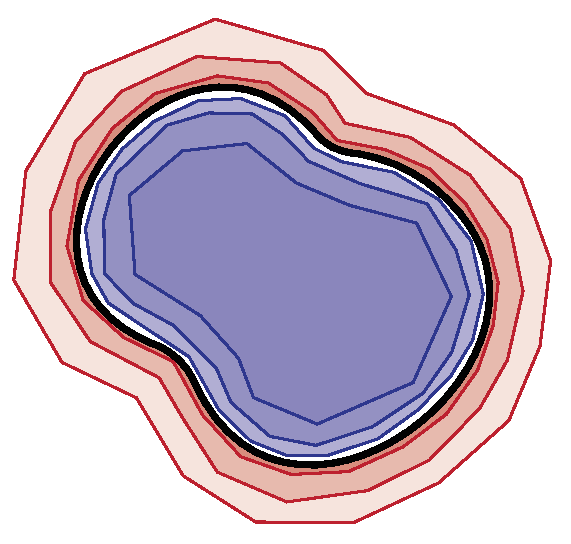
\includegraphics[trim=0cm 0cm 0cm 0cm, clip, scale=0.71]{images/peanopoligoni.pdf}
\end{center}
Se l'estremo inferiore dei poligoni esterni coincide con quello superiore di quelli interni, potremmo dire che l'insieme è misurabile e ha area pari a questo limite.
Inoltre, Peano fornisce una condizione necessaria e sufficiente: la differenza tra i poligoni esterni ed interni deve essere piccola a piacere, ossia la frontiera dell'insieme (che chiaramente è contenuta nell'area di piano fra i poligoni esterni ed interni) dovrà avere misura nulla.\\
Possono capitare anche insiemi che non ammettono area. 
\begin{example}
	Supponiamo di prendere tutti i punti a distanza \textit{razionale} $r\leq 1$ dall'origine, cioè infinite circonferenze di raggio razionale interne al disco di raggio 1.\\
	Chiaramente l'area interna è uguale a 0, mentre essendo l'insieme denso nel disco di raggio 1, ogni poligono che la contiene contiene il cerchio e quindi l'area esterna è maggiore o uguale 1: essendo l'area interna e l'area esterna diverse, il poligono non ammette aree.
\end{example}
La misura di Peano, per quanto innovativa, risente di alcuni problemi: parlare di poligoni o solidi poligonali è facile farlo in $\realset^2$ o $\realset^3$, ma non è generalizzabile in dimensioni maggiori: ad esempio, qual è la misura di un ipersolido poligonale di dimensione 4? Inoltre, la misura di Peano non è numerabilmente additiva, ossia un'unione \textit{infinita numerabile} di insiemi misurabili secondo Peano non è necessariamente ancora misurabile.\\
Qualche anno dopo i lavori di Peano, il matematico francese Marie Camille \textbf{Jordan} (1838-1922) \textit{estende} il concetto di misura introdotta da Peano a una generica dimensione $n$, utilizzando invece che poligoni o solidi poligoni delle \textit{unioni di intervalli}, \textit{rettangoli} o, in generale, \textit{parallelepipedi} $n$-dimensionali, poiché questi hanno una misura ben nota!
\begin{center}
	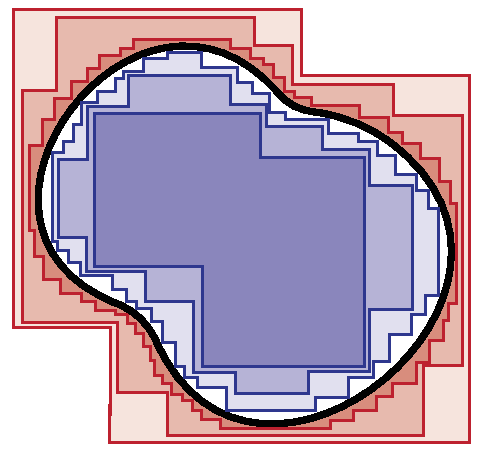
\includegraphics[trim=0cm 0cm 0cm 0cm, clip, scale=0.71]{images/peanoparallelepipedi.pdf}
\end{center}
Anche se questa misura coincide con quella di Peano (dopotutto, le unioni di parallelepipedi sono un \textit{caso particolare} di ipersolidi poligonali), in questo modo si risolve il \textit{primo problema} dei due problemi enunciati precedentemente; ciò nonostante, questa definizione non è ancora una misura numerabilmente-additiva.
\subsection{Definizione e osservazioni sulla misura di Peano-Jordan}
\begin{define}[Parallelepipedo {$n$}-dimensionale]
	Un \textbf{parallelepipedo}\index{parallelepipedo} $n$-dimensionale è un \textit{plurintervallo}, ossia un prodotto cartesiano di $n$ intervalli:
	\begin{equation}
		P=\prod_{i=1}^{n}\left[a_i,b_i\right]\quad\text{con }-\infty < a_i < b_i < +\infty
	\end{equation}
	Posta la \textbf{lunghezza}\index{lunghezza!di un intervallo} di un intervallo come
		\begin{equation}
			\mathcal{L}\left(\left[a_i,b_i\right]\right)=b_i-a_i
		\end{equation}
		la misura $n$-dimensionale del parallelepipedo è
		\begin{equation}
			V_n\left(P\right)=\prod_{i=1}^{n}\mathcal{L}\left(\left[a_i,b_i\right]\right)
		\end{equation}
	\end{define}
	Introduciamo formalmente la misura esterna e la misura interna di un insieme limitato $A$ come estremi inferiori e superiori di un \textbf{insieme elementare}\index{insieme!elementare}, cioè un'unione finita di parallelepipedi:
	\begin{itemize}
		\item \textsc{Misura esterna}:\index{misura!esterna} \begin{equation}
			m_{PJ}^X\left(A\right)=\inf\left\{\sum_{i=1}^{n}V_n\left(P_i\right)\mid P_i\text{ parallelepipedi},\ \bigcup_{i=1}^nP_i\supseteq A\right\}
		\end{equation}
		\item \textsc{Misura interna}:\index{misura!interna}
		\begin{equation}
			m_{PJ,X}\left(A\right)=\inf\left\{\sum_{i=1}^{n}V_n\left(P_i\right)\mid P_i\text{ parallelepipedi},\ \bigcup_{i=1}^nP_i\subseteq A\right\}
		\end{equation}
	\end{itemize}
	In generale $m_{PJ,X}\left(A\right)\leq m_{PJ}^{X}\left(A\right)$.
	\begin{define}[Misura di Peano-Jordan]
		Un insieme limitato $A$ è \textbf{misurabile secondo Peano-Jordan}\index{misura!secondo Peano-Jordan} se
		\begin{equation}
			m_{PJ}^X\left(A\right)=m_{PJ,X}\left(A\right)
		\end{equation}
	e la \textbf{misura} (secondo P-J) dell'insieme è
		\begin{equation}
			m_{PJ}\left(A\right)=m_{PJ}^X\left(A\right)=m_{PJ,X}\left(A\right)
		\end{equation}
	\end{define}
	\begin{propositionqed}[Criterio di misurabilità]
		L'insieme limitato $A\subseteq \realset^n$ è misurabile per Peano-Jordan se e solo se $\forall \epsilon>0,\ \exists P\subseteq A, Q\supseteq A$ con $P,\ Q$ insiemi elementari tali che
		\begin{equation}
			m_{PJ}\left(Q\right)-m_{PJ}\left(P\right)\leq \epsilon\qedhere
		\end{equation}
	\end{propositionqed}
	Definito
	\begin{equation}
		\mathcal{M}=\left\{A\subseteq \realset^n\mid A\text{è P-J misurabile}\right\}
	\end{equation}
	essa è un'\textit{algebra}, \textit{ma} non una $\sigma$-algebra, cioè non è chiusa rispetto all'unione \textit{numerabile infinita}.
	\begin{examplewt}[Controesempio dell'additività numerabile della misura di P-J]
		Consideriamo
		\begin{equation*}
			E=\rationalset\cap\left[0,1\right]=\bigcup_{n\geq 1}\left\{r_n\right\}
		\end{equation*}
		dove $\left\{r_n\right\}$ è un'enumerazione di razionali in $\left[0,1\right]$.\\
		$\left\{r_n\right\}$ è un punto e dunque è misurabile con misura nulla, ma \begin{equation*}
			\bigcup_{n\geq 1}\left\{r_n\right\}=E
		\end{equation*}
		\textit{non} è misurabile, dato che
		\begin{equation*}
			\begin{cases}
				m_{PJ}^X\left(E\right)=1\\
				m_{PJ,X}\left(E\right)=0
			\end{cases}
		\end{equation*}
	\end{examplewt}
	In altre parole, la misura secondo Peano-Jordan è \textit{additiva}, ma non $\sigma$-additiva.
	\begin{digression}
		Nella letteratura italiana si è soliti parlare ‘‘misura di Peano-Jordan'', quando in realtà questa terminologia è impropria, non essendo una \textit{misura} nel senso \textit{moderno} del termine. Nell'anglosfera lo stesso concetto viene chiamato ‘‘Jordan content'.
	\end{digression}
	\section{Misura secondo Lebesgue}
	Per quanto innovativa, la misura di Peano-Jordan presenta alcuni notevoli problemi:
	\begin{itemize}
		\item É definita solo per \textit{insiemi limitati}.
		\item Non è \textit{numerabilmente additività}: la misura di un'unione numerabilmente infinita di insiemi misurabili non è necessariamente misurabile.
	\end{itemize}
	Il concetto \textit{moderno} di misura di un sottoinsieme dello spazio $n$-dimensionale viene per la prima volta presentato in \textit{Intégrale, longueure, aire} (1902)
	dal matematico francese Henri \textbf{Lebesgue} (1875-1941) nell'ambito dell'annoso problema delle discontinuità nell'integrale definito.\\
	La costruzione della misura secondo Lebesgue inizia in modo analogo a quella di Peano-Jordan, definendo i \textit{parallelepipedi}; per poter definire la misurabilità di insiemi illimitati si ammettono parallelepipedi \textit{degeneri}.
	\begin{define}[Parallelepipedo {$n$}-dimensionale]
		Un \textbf{parallelepipedo}\index{parallelepipedo} $n$-dimensionale è un \textit{plurintervallo}, ossia un prodotto cartesiano di $n$ intervalli eventualmente \textit{degeneri}:
		\begin{equation}
			P=\prod_{i=1}^{n}\left[a_i,b_i\right]\quad\text{con }-\infty \leq a_i \leq b_i \leq +\infty
		\end{equation}
		Posta la \textbf{lunghezza}\index{lunghezza!di un intervallo} di un intervallo come
		\begin{equation}
			\mathcal{L}\left(\left[a_i,b_i\right]\right)=
			\begin{cases}
				\begin{array}{ll}
					b_i-a_i & \text{se }-\infty < a_i \leq b_i < +\infty\\
					+\infty&\text{altrimenti}
				\end{array}
			\end{cases}
		\end{equation}
		la misura $n$-dimensionale del parallelepipedo è
		\begin{equation}
			V_n\left(P\right)=\prod_{i=1}^{n}\mathcal{L}\left(\left[a_i,b_i\right]\right)
		\end{equation}
		con la convenzione che $0\cdot \infty =0$.
	\end{define}
	\begin{observe}
		Come mai $0\cdot \infty$ non è lasciato indeterminato, ma posto proprio uguale a 0?. Per capirlo, facciamo prima un esempio in dimensione 2; consideriamo il rettangolo degenere
		\begin{equation*}
			P=\left\{a_1\right\}\times\left(a_2,+\infty\right).
		\end{equation*}
		Esso è un sottoinsieme di $\realset^2$, ma ha chiaramente una sola dimensione: seppur come semiretta ha una lunghezza ben definita (e in tal caso sarebbe infinita tale lunghezza), è ragionevole dire che come oggetto \textit{bidimensionale} abbia \textit{area} $0$.
		\begin{center}
			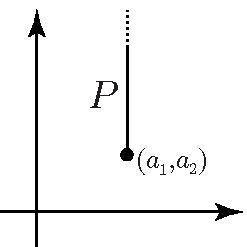
\includegraphics[trim=0cm 0cm 0cm 0cm, clip, scale=0.71]{images/rettangolodegenere.pdf}
		\end{center}
		In altre parole, se almeno un intervallo che compone il parallelepipedo $n$-dimensionale ha lunghezza nulla, $P$ è da intendersi come elemento di dimensione $k$ in uno spazio $n$-dimensionale, con $k< n$.
		In questo caso, la sua misura $n$\textit{-dimensionale} è nulla, anche se fosse \textit{illimitato} in diverse direzioni, da qui spiegato il perché di $0\cdot \infty =0$.
	\end{observe}
	A differenza di Peano-Jordan, Lebesgue definisce solamente la \textbf{misura esterna} dell'insieme:
	\begin{equation}
		m^X\left(A\right)=\inf\left\{\sum_{i=1}^{n}V_n\left(P_i\right)\middle| P_i\text{ parallelepipedi aperti},\ \bigcup_{i=1}^nP_i\supseteq A\right\}
	\end{equation}
dove per parallelepipedo \textit{aperti} si intende un plurintervallo definito da intervalli aperti.\\ 
	Essa si può vedere come una funzione
	\begin{equation}
		\funz{m^X}{\setpart{\realset^n}}{\left[0,+\infty\right]}
	\end{equation}
	che gode delle seguenti proprietà:
	\begin{itemize}
		\item Se l'insieme è un parallelepipedo $n$-dimensionale, la misura esterna del parallelepipedo ovviamente coincide con la misura $n$-dimensionale di esso:
		\begin{equation}
			m^X\left(P\right)=V_n\left(P\right),\ \forall P\text{ parallelepipedo}
		\end{equation}
		\item È \textit{monotona}:
		\begin{equation}
			m^X\left(A\right)\leq m^X\left(B\right),\ \forall A\subseteq B
		\end{equation}
		\item È $\sigma$-\textit{subadditiva}:
		\begin{equation}
			m^X\left(\bigcup_{n\geq 1}A_n\right)\leq \sum_{n\geq 1}m^X\left(A_n\right), \forall A_n\subseteq \realset^n
		\end{equation}
		\item È \textit{invariante per traslazioni}:
		\begin{equation}
			m^X\left(A+\left\{x\right\}\right)=m^X\left(A\right),\ \forall x\in\realset^n,\ \forall A\subseteq\realset^n
		\end{equation}
	\end{itemize}
	Osserviamo che per $m^X$ vale \textit{solo} la  $\sigma$-\textit{subadditività}, ma non la $\sigma$-\textit{additività}.
	\begin{define}[Insieme misurabile secondo Lebesgue {{\small (Criterio di Caratheodory)}}]\index{criterio!di Caratheodory}
		Un insieme $A\subseteq\realset^n$ è \textbf{misurabile secondo Lebesgue} se $\forall E\subseteq\realset^n$ vale
		\begin{equation}
			m_n^X\left(E\right)=m_n^X\left(E\cap A\right)+m_n^X\left(E\cap A^C\right)
		\end{equation}
	\end{define}
	$E$ è un \textbf{insieme test}\index{insieme!test} arbitrario (non necessariamente misurabile!): $A$ è misurabile se decompone bene $E$ in due sottoinsiemi misurabili $E\cap A$ e $E\cap A^C$.
	\begin{center}
		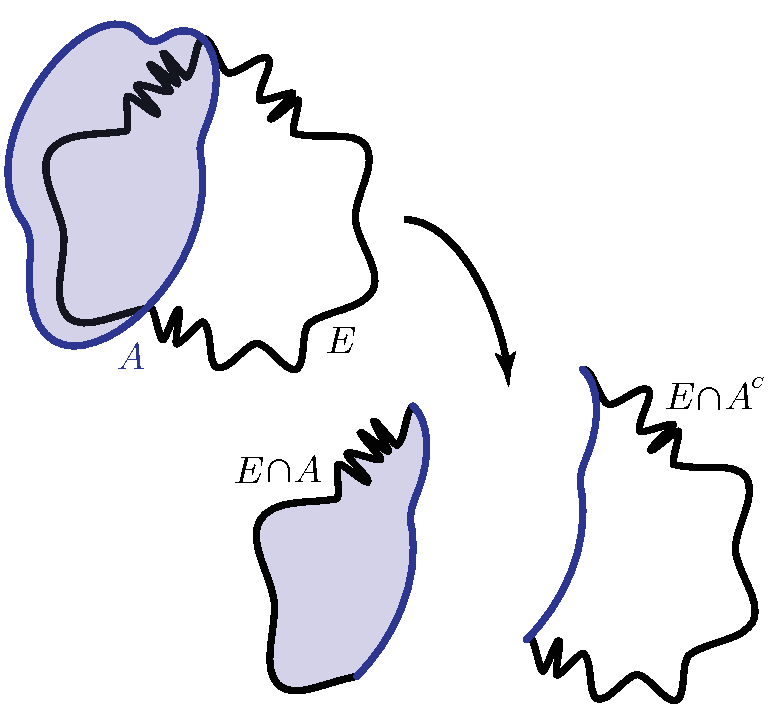
\includegraphics[trim=0cm 0cm 0cm 0cm, clip, scale=0.5]{images/criteriomisurabilita.pdf}
	\end{center}
	\begin{propositionqed}[Gli insiemi misurabili secondo Lebesgue sono una {$\sigma$}-algebra]
		La collezione di insiemi
		\begin{equation*}
			\mathcal{L}\left(\realset^n\right)=\left\{A\subseteq \realset^n\mid A\text{ è Lebesgue-misurabile}\right\}
		\end{equation*}
		è una $\sigma$-algebra.
	\end{propositionqed}
	\begin{define}[Misura secondo Lebesgue]
		La \textbf{misura secondo Lebesgue}\index{misura!secondo Lebesgue} è la restrizione della misura esterna a $\mathcal{L}\left(\realset^n\right)$:
		\begin{equation}
			m_n={m^X_n}\vert_{ \mathcal{L}\left(\realset^n\right)}\text{ ossia }\funz{m_n}{\mathcal{L}\left(\realset^n\right)}{\left[0,+\infty\right]}
		\end{equation}
	\end{define}
\subsection{Insiemi misurabili secondo Lebesgue}
La definizione data di insieme misurabile secondo Lebesgue non è particolarmente \textit{operativa}, in quanto richiede di controllare che un generico insieme test decomponga bene l'insieme di cui vogliamo verificare la misurabilità.
Di seguito presentiamo alcune classi importanti di insiemi misurabili secondo Lebesgue.
\begin{itemize}
	\item \textsc{\textbf{Insiemi elementari:}} (unioni di) parallelepipedi, anche degeneri:
	\begin{gather*}
		m_n\left(P\right)=V_n\left(P\right)\\
		m_n\left(\bigcup_{i=1}^{+\infty} P_i\right)=\sum_{i=1}^{+\infty}V_n\left(P_i\right)
	\end{gather*}
In particolare:
\begin{itemize}
	\item Preso $P=\realset^n$, allora $m_n\left(\realset^n\right)=+\infty$.
	\item Preso $P=\left\{x\right\},\ \forall x\in\realset^n$, allora $m_n\left(\left\{x\right\}\right)=0$.
\end{itemize}
\item \textsc{\textbf{Borelliani:}} $\mathcal{B}\left(\realset^n\right)\subsetneqq\mathcal{L}\left(\realset^n\right)$.\\
È importante sottolineare che ci sono insiemi misurabili \textit{non} Borelliani.
% TO DO: aggiungere esempio quando ci sarà l'occasione.
\item \textsc{\textbf{Tutti gli insiemi aventi misura \textit{esterna} nulla:}}
\begin{equation*}
	\forall A\subseteq \realset^n\ m_n^X\left(A\right)=0\implies A\in\mathcal{L}\left(\realset^n\right)\text{ e }m_n\left(A\right)=0
\end{equation*}
\end{itemize}

\begin{demonstration}
	Dobbiamo provare che $\forall E\subseteq \realset^n$
	\begin{equation*}
		m_n^X\left(E\right)=m_n^X\left(E\cap A\right)+m_n^X\left(E\cap A^C\right)
	\end{equation*}
	Ricordiamo che $m_n^X$ è $\sigma$-subadditiva e quindi finito-subadditiva, quindi
	\begin{equation*}
		E=\left(E\cap A\right)\cup \left(E\cap A^C\right)\implies m_n^X\left(E\right)\leq m_n^X\left(E\cap A\right)+m_n^X\left(E\cap A^C\right)
	\end{equation*}
	È sufficiente allora provare la disuguaglianza opposta. Osserviamo che $E\cap A^C\subseteq E$, dunque per monotonia di $m_n^X$ si ha
	\begin{equation*}
		m_n^X\left(E\right)\geq m_n^X\left(E\cap A^C\right)=m_n^X\left(E\cap A^C\right)+0=m_n^X\left(E\cap A^C\right)+m_n^X\left(E\cap A\right)
	\end{equation*}
	Infatti $E\cap A\subseteq A$ implica, per monotonia di $m_n^X$ che
	\begin{equation*}
		0\leq m_n^X\left(E\cap A\right)\leq m_n^X\left(A\right)=0
	\end{equation*}
	e quindi $m_n^X\left(E\right)\geq m_n^X\left(E\cap A^C\right)+m_n^X\left(E\cap A\right)$.
\end{demonstration}
\begin{attention}
	\textbf{Non} tutti gli insiemi sono misurabili! Se supponiamo vero l'Assioma della Scelta, l'\textbf{insieme di Vitali} è un insieme non misurabile in $\realset$ rispetto alla misura di Lebesgue unidimensionale\footnote{Si veda pag. \pageref{vitali} per la definizione dell'insieme di Vitali e la dimostrazione di ciò.}.
\end{attention}
Nella teoria di Lebesgue hanno un ruolo importante gli insiemi di misura nulla: esplicitiamo il legame tra misura nulla e cardinalità.
È noto che ogni singolo punto ha misura nulla; osserviamo che presa una famiglia di punti $\left\{x_n\right\}$ si ha
\begin{equation*}
	0\leq m_n\left(\bigcup_{n\geq 1}\left\{x_n\right\}\right)\leq \sum_{n\geq 1}m_n\left(\left\{x_n\right\}\right)=0
\end{equation*}
Ogni insieme \textbf{numerabile} è misurabile e ha misura nulla.
\begin{example}
	Posto $n=1$, ossia consideriamo la misura in $\realset$, si ha
	\begin{equation*}
		m_1\left(\rationalset\right)=0,\ m_1\left(\rationalset\cap\left[0,1\right]\right)=0
	\end{equation*}
\end{example}
\subsubsection{L'insieme (ternario) di Cantor}\label{insiemecantor}
Esistono anche insiemi di misura nulla con \textit{cardinalità del continuo}. Uno di questi è l'\textbf{insieme ternario di Cantor}, il quale possiede diverse proprietà interessanti e non particolarmente immediate. Esso si costruisce partendo dall'intervallo $\left[0,1\right]$ con il seguente procedimento iterativo:
\begin{itemize}
	\item \textbf{Passo 0.} È semplicemente l'intervallo $\left[0,1\right]$.
	\begin{center}
		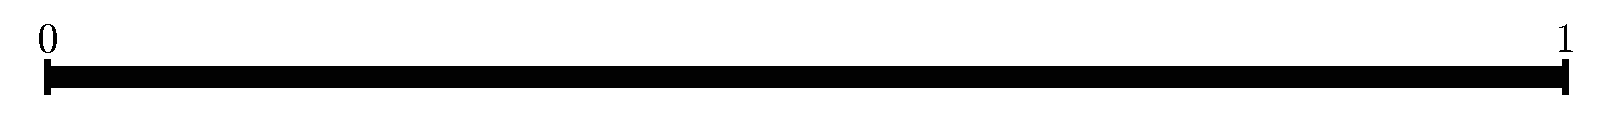
\includegraphics[trim=0cm 0cm 0cm 0cm, clip, scale=0.5]{images/Cantor0.pdf}
	\end{center}
	\item \textbf{Passo 1.} Suddividiamo $\left[0,1\right]$ in tre sottointervalli di ugual lunghezza
	\begin{equation*}
		I_1=\left[0,\nicefrac{1}{3}\right]\qquad I_2=\left(\frac{1}{3},\nicefrac{2}{3}\right)\qquad I_3=\left[\frac{2}{3},1\right]
	\end{equation*}
	e rimuoviamo l'intervallo aperto intermedio $I_2$, lasciando gli intervalli $I_1$ e $I_2$.
	\begin{center}
		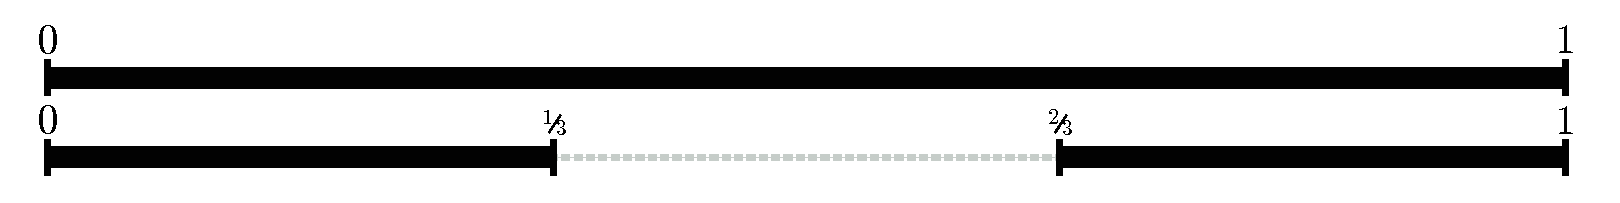
\includegraphics[trim=0cm 0cm 0cm 0cm, clip, scale=0.5]{images/Cantor1.pdf}
	\end{center}
	\item \textbf{Passo 2.} Prendiamo ciascun intervallo che avevamo al passo 1 e lo suddividiamo in modo analogo in tre parti uguali; per ciascun intervallo eliminiamo il sottointervallo aperto centrale, lasciando dunque 4 intervalli di lunghezza $\nicefrac{1}{9}$.
	\begin{center}
		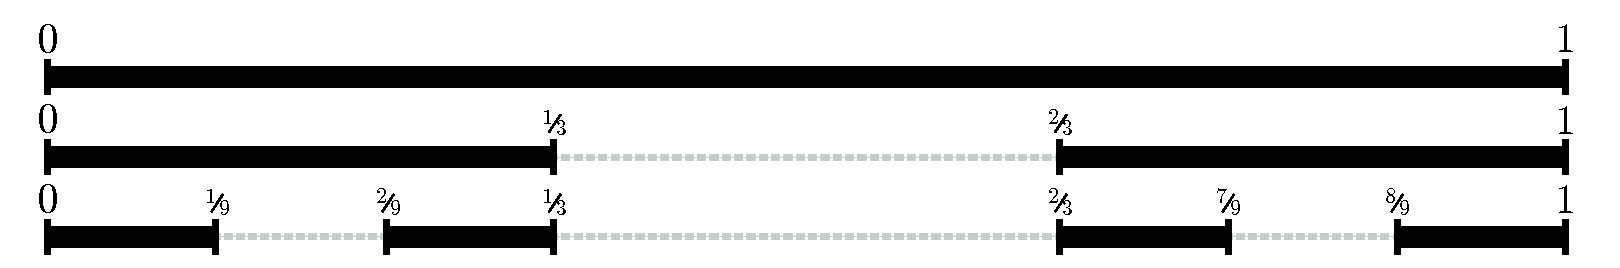
\includegraphics[trim=0cm 0cm 0cm 0cm, clip, scale=0.5]{images/Cantor2.pdf}
	\end{center}
	\item \textbf{Passo 3 e successivi.} Ripetiamo il procedimento del passo 2 con gli intervalli ottenuti nel passaggio precedente.
\begin{center}
	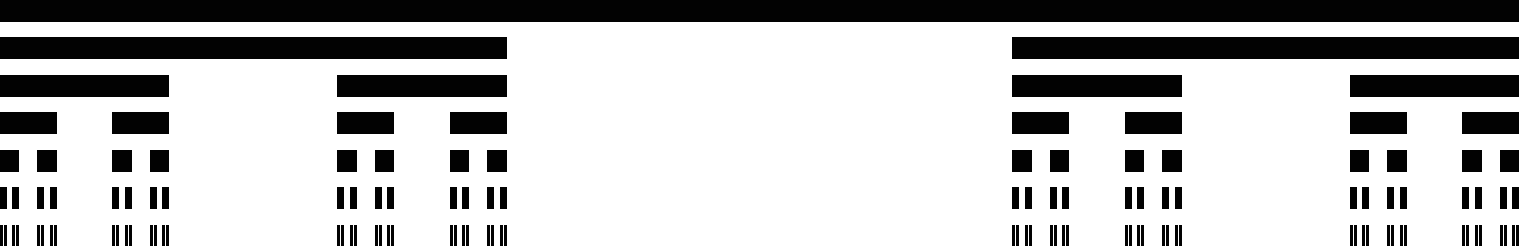
\includegraphics[trim=0cm 0cm 0cm 0cm, clip, scale=0.5]{images/Cantor3.pdf}
\end{center}
\end{itemize}
I punti che rimangono dopo infiniti passi è noto come \textbf{insieme di Cantor}\index{insieme!di Cantor} $C$.\\
Ci si potrebbe chiedere se ci sono ancora dei punti in questo insieme: dopotutto, abbiamo rimosso e rimosso continuamente degli intervalli. Sorprendentemente, dopo infiniti di questi passi ci sono ancora punti che rimangono, ma la peculiarità è che sono addirittura \textbf{non numerabili}!
\begin{theorema}[Innumerabilità dell'insieme di Cantor]
	Si denoti con $C$ l'insieme ternario di Cantor. Esiste una funzione suriettiva da $C$ in $\left[0,1\right]$; conseguentemente, $C$ ha la cardinalità del continuo.
\end{theorema}
\begin{demonstration}
	Ricordiamo che per ogni numero $x\in [0,1]$ esiste una successione $\{i_n\}_{n\geq 1}$ di interi, con $i_n\in \{0, 1, 2\}$, tale che 
	\begin{equation*}
		x=\sum_{n=1}^{+\infty} \dfrac{i_n}{3^n}. 
	\end{equation*}
	Tale successione è unica, tranne quando $x$ è della forma $q/3^n$, con  $q\in \naturalset$, nel qual caso esistono esattamente due successioni.\\
	Descriviamo l'insieme di Cantor $C$ usando questa rappresentazione in base tre.\\
	Osserviamo che $\nicefrac{1}{3}$ si scrive come $0.1_3$ e $\nicefrac{2}{3}$ si scrive come $0.2_3$; il primo intervallo rimosso nella costruzione dell'insieme di Cantor consiste quindi di tutti i numeri del tipo $0.1abc\ldots_3$, dove $abc\ldots$ è una qualsiasi sequenza di numeri diversi dalle sequenze estreme $0000\ldots$ e $222\ldots$.\\
	I numeri residui dopo il primo passo della costruzione di $C$ sono esattamente quelli scrivibili come $0.0abc\ldots_3$ e $0.2abc\ldots_3$.\\
	Al secondo passo si rimuovono tutti i numeri del tipo $0.01abc\ldots_3$ e $0.21abc\ldots_3$ e così via: segue che i numeri che non vengono mai rimossi e che quindi appartengono all'insieme $C$ sono esattamente quelli che possono essere scritti come $0.abc\ldots_3$ usando solo le cifre $0$ e $2$.\\
	Definiamo ora una funzione $\funz{f}{C}{\left[0,1\right]}$ associando ad ogni elemento di $C$ scritto come $0.abc\ldots_3$, dove le cifre decimali sono solo $0$ e $2$, il numero di $\left[0,1\right]$ la cui rappresentazione in base due è quella ottenuta dalla sequenza $0.abc\ldots$ sostituendo ogni cifra $2$ con la cifra $1$.\\
	La funzione $f$ è chiaramente suriettiva: dato un numero $x\in \left[0,1\right]$, la sua controimmagine mediante $f$ è l'elemento dell'insieme di Cantor la cui rappresentazione decimale ternaria si ottiene dalla rappresentazione binaria di $x$ sostituendo ogni cifra $1$ con la cifra $2$.\\
	L'esistenza di una funzione suriettiva da $C$ in $\left[0,1\right]$ implica\footnote{In ‘‘Brevi cenni di teoria degli insiemi'', a pag. \pageref{cardinalitàsuriettiva} è possibile trovare maggiori dettagli su questa proprietà.} che la cardinalità di C è maggiore o uguale a quella di $\left[0,1\right]$:
	\begin{equation*}
		\abs{C}\geq \abs{X} 
	\end{equation*}
	D'altra parte, $C\subseteq \left[0,1\right]$ e dunque\footnote{In ‘‘Brevi cenni di teoria degli insiemi'', a pag. \pageref{cardinalitàinclusione} è possibile trovare maggiori dettagli su questa proprietà.} la sua cardinalità è minore o uguale a quella di $\left[0,1\right]$.
	\begin{equation*}
		\abs{C}\leq\abs{X}
	\end{equation*}
	Concludiamo quindi che $C$ e $\left[0,1\right]$ hanno la stessa cardinalità e dunque $C$ ha la cardinalità del continuo $\mathfrak{c}$.
\end{demonstration}
\begin{digression}
	Si noti che l'insieme di Cantor è un \textbf{frattale}\index{frattale}, dato che è sempre uguale a due copie di se stesso, se ogni copia è ristretta di un terzo e traslata.
\end{digression}
Pur essendo non numerabile esso ha lunghezza nulla. Nello specifico, consideriamo la misura di Lebesgue $m_1$ e ripercorriamo i passaggi della costruzione dell'insieme di Cantor:
\begin{itemize}
	\item \textbf{Passo 0.} $C_0$ coincide con l'intervallo $\left[0,1\right]$:
	\begin{equation*}
		m_1\left(C_0\right)=1
	\end{equation*}
	\item \textbf{Passo 1.} Togliamo un segmento di lunghezza $\nicefrac{1}{3}$ da un segmento di lunghezza $1$:
	\begin{equation*}
		m_1\left(C_1\right)=m_1\left(C_0\right)-\frac{1}{3}=\frac{2}{3}
	\end{equation*}
	\item \textbf{Passo 2.} Togliamo dei segmenti di lunghezza complessiva $\nicefrac{2}{9}$ da un'unione di segmenti di lunghezza $\nicefrac{2}{3}$:
	\begin{equation*}
		m_1\left(C_2\right)=m_1\left(C_1\right)-\frac{2}{9}=\frac{2}{3}-\frac{2}{9}=\frac{4}{9}
	\end{equation*}
\end{itemize}
Ad ogni passo l'insieme ha sempre lunghezza $\nicefrac{2}{3}$ quello del precedente. Al passo $n$-esimo si ha
\begin{equation*}
	m_1\left(C_n\right)=\left(\frac{2}{3}\right)^n
\end{equation*}
Poiché l'insieme di Cantor è prodotto dopo infiniti passi, allora
\begin{equation*}
	m_1\left(C\right)=\lim_{n\to+\infty}m_1\left(C_n\right)=\lim_{n\to+\infty}\left(\frac{2}{3}\right)^n=0
\end{equation*}
\subsection{Regolarità della misura di Lebesgue}
Ora enunciamo una proprietà della misura di Lebesgue, detta \textbf{regolarità}\index{regolarità!della misura di Lebesgue}.
\begin{theorema}[Regolarità della misura di Lebesgue]\label{regolaritàlebesgue}
	Le seguenti affermazioni sono equivalenti:
	\begin{enumerate}
		\item $E\in\mathcal{L}\left(\realset^n\right)$.
		\item $\forall \epsilon > 0,\ \exists A_{\epsilon}$ aperto di $\realset^n$ tale che
		\begin{itemize}
			\item $E\subseteq A_{\epsilon}$.
			\item $m^{X}_n\left(A_{\epsilon}\setminus E\right)<\epsilon$.
		\end{itemize}
		\item $\exists B$ Borelliano di $\realset^n$ tale che
	\begin{itemize}
		\item $E\subseteq B$.
		\item $m^{X}_n\left(B\setminus E\right)=0$.
	\end{itemize}
	\item $\forall \epsilon > 0,\ \exists C_{\epsilon}$ chiuso di $\realset^n$ tale che
	\begin{itemize}
		\item $E\supseteq C_{\epsilon}$.
		\item $m^{X}_n\left(E\setminus C_{\epsilon}\right)<\epsilon$.
	\end{itemize}
	\item $\exists D$ Borelliano di $\realset^n$ tale che
	\begin{itemize}
		\item $E\supseteq D$.
		\item $m^{X}_n\left(E\setminus D\right)=0$.
	\end{itemize}~\\
	\begin{minipage}{0.4\textwidth}
	\begin{center}
		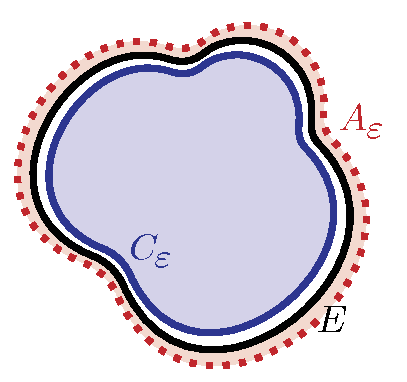
\includegraphics[trim=0cm 0cm 0cm 0cm, clip, scale=0.7]{images/regolarita1}\\
		\textbf{Caso 2. + 4.}
	\end{center}
\end{minipage}
\begin{minipage}{0.5\textwidth}
	\begin{center}
			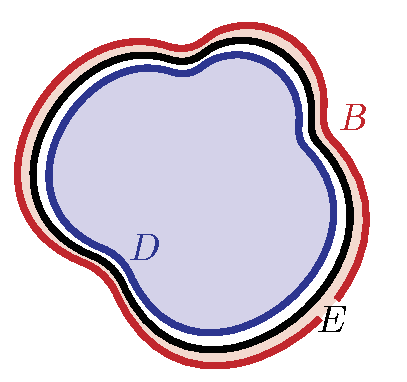
\includegraphics[trim=0cm 0cm 0cm 0cm, clip, scale=0.7]{images/regolarita2}\\
			\textbf{Caso 3. + 5.}
	\end{center}
\end{minipage}
	\end{enumerate}
\end{theorema}
\begin{demonstration}
	Dimostriamo le catene di implicazioni
	\begin{equation*}
		\mathbf{(i)\implies (ii)\implies (iii)\implies (i)\qquad(i)\implies (iv)\implies (v)\implies (i)}
	\end{equation*}
$\mathbf{(i)\implies(ii)}\quad$ Consideriamo il caso $m_n\left(E\right)<+\infty$. Per definizione di $m^{X}_n$ e di $\inf$, fissato $\epsilon >0$ $E$ è contenuto in un ricoprimento di parallelepipedi aperti tale che
\begin{equation*}
	\sum_{i=1}^{+\infty}V_n\left(P_i\right)<m_n\left(E\right)+\epsilon
\end{equation*}
dunque, posto
\begin{equation*}
	A=\bigcup_{n\in\naturalset}P_n,
\end{equation*}
l'aperto $A$ verifica, per subadditività numerabile,
\begin{equation*}
	m_n\left(A\right)<m_n\left(E\right)+\epsilon
\end{equation*}
e dal fatto che $m_n\left(E\right)<+\infty$ segue allora % aggiungere tabella proprietà in footnotes
\begin{equation*}
	m_n\left(A\setminus E\right)=m_n\left(A\right)-m_n\left(E\right)<\epsilon
\end{equation*}
Sia ora $m_n\left(E\right)=+\infty$. Possiamo vederlo come la seguente unione:
\begin{equation*}
	E=\bigcup_{i=1}^{+\infty}\left(E\cap Q_i\right),
\end{equation*}
dove $Q_i$ è una famiglia di parallelepipedi privi di punti interni comuni (ossia che hanno in comune al più i bordi), la cui unione sia $\realset^n$. Dato che $m_n\left(E\cap Q_n\right)<m_n\left(E\right)<Q$, per quanto già dimostrato esistono degli $A_i\supseteq E\cap Q_i$ tali che
\begin{equation*}
	m_n\left(A_i\setminus\left(E\cap Q_i\right)\right)<\frac{\epsilon}{2^{i+1}},\ \forall i\in\naturalset
\end{equation*}
Allora possiamo prendere come aperto
\begin{equation*}
	A=\bigcup_{i=1}^{+\infty}A_i.
\end{equation*}
Esso contiene $E$, e poiché
\begin{equation*}
	A\setminus E=\left(\bigcup_{i=1}^{+\infty}A_i\right)\setminus\left(\bigcup_{i=1}^{+\infty}\left(E\cap Q_i\right)\right)\subseteq\bigcup_{i=1}^{+\infty}\left(A_i\setminus\left(E\cap Q_i\right)\right)
\end{equation*}
si conclude che
\begin{equation*}
	m_n\left(A\setminus E\right)<\sum_{i=1}^{+\infty}m_n\left(A_i\setminus\left(E\cap Q_i\right)\right)<\epsilon
\end{equation*}
$\mathbf{(ii)\implies(iii)}\quad$ Per ogni $i\in\naturalset$, sia $A_i$ un aperto contenente $E$, tale che
\begin{equation*}
	m^{X}_n\left(A_i\setminus E\right)<\frac{1}{i+1}.
\end{equation*}
L'insieme
\begin{equation*}
	B=\bigcap_{i=1}^{+\infty}A_i
\end{equation*}
è un borelliano contenente $E$ e si ha, per monotonia,
\begin{equation*}
	m_n^{X}\left(B\setminus E\right)\leq m_n^{X}\left(A_i\setminus E\right)<\frac{1}{n+1},\ \forall i\in \naturalset
\end{equation*}
cioè $m_n^{X}\left(B\setminus E\right)=0$.\\
$\mathbf{(iii)\implies(i)}\quad$  Scrivendo $E=B\setminus\left(B\setminus E\right)$, la tesi segue dal fatto che l'insieme $B$ è misurabile perché boreliano, mentre l'insieme $B\setminus E$ è misurabile avendo, per ipotesi, misura esterna nulla. Dunque $E$ è misurabile.\\
$\mathbf{(i)\implies(iv)\implies(v)\implies(i)}\quad$ Queste implicazioni si dimostrano facilmente applicando ad $E^C$ gli enunciati già dimostrati. 
\end{demonstration}
\begin{observe}
	Dai punti 2 e 4 si può caratterizzare un insieme $E$ misurabile secondo Lebesgue come un insieme che \textit{differisce poco}, in termini della misura esterna, sia da aperti contenenti $E$, sia da chiusi contenuti in $E$.\\
	Dai punti 3 e 5, invece, si può vedere ogni insieme misurabile secondo Lebesgue come un Borelliano a cui abbiamo tolto o aggiunto, rispettivamente, un insieme di misura nulla. Nello specifico, dal punto 5,
	\begin{equation*}
		E=D\cup\left(E\setminus D\right)
	\end{equation*}
\end{observe}
\subsection{Confronto tra la misura di Peano-Jordan e di Lebesgue}
Come abbiamo visto, la misura di Peano-Jordan soddisfa solo alcune proprietà della misura in senso assiomatico, essendo $\sigma$-subadditiva, mentre la misura secondo Lebesgue è a tutti gli effetti una misura assiomatica moderna. Ci si può dunque chiedere se tali concetti sono incompatibili tra di loro oppure se c'è una qualche relazione tra di esse.\\
È già noto che non tutti gli insiemi misurabili secondo Lebesgue lo sono secondo Peano-Jordan.
\begin{example}
	Consideriamo $E=\rationalset\cap\left[0,1\right]$.
	\begin{itemize}
		\item $E$ numerabile implica che $E$ è Lebesgue-misurabile e $m_1\left(E\right)=0$.
		\item $E$ \textit{non} è Peano-Jordan misurabile, in quanto
		\begin{equation*}
			m_{PJ}^{X}\left(E\right)=1\neq 0=m_{PJ,X}\left(E\right)
		\end{equation*}
	\end{itemize}
\end{example}
Invece, si vede banalmente che gli insiemi elementari, ossia le unioni di parallelepipedi $n$-dimensionali, sono misurabili sia secondo Lebesgue, sia secondo Peano-Jordan (a patto di fare un'unione finita di elementi); in particolare, le misure coincidono.
\begin{gather*}
	m_{PJ}\left(P\right)=m_n\left(P\right)=V_n\left(P\right)\\
	m_{PJ}\left(\bigcup_{i=1}^{k}P_i\right)=m_n\left(\bigcup_{i=1}^{k}P_i\right)=\sum_{i=1}^{k}V_n\left(P_i\right)
\end{gather*}
Il seguente teorema ci afferma un risultato importante: \textit{tutti} gli insiemi misurabili secondo Peano-Jordan sono misurabili secondo Lebesgue e le misure in tal caso coincidono.
\begin{theorema}[Misurabile secondo Peano-Jordan implica misurabile secondo Lebesgue]
	Sia $E\subseteq\realset^n$ limitato. Allora
	\begin{enumerate}
		\item Se $E$ è Peano-Jordan misurabile allora $E$ è Lebesgue misurabile.
		\item Se vale ciò, allora $m_{PJ}\left(E\right)=m_n\left(E\right)$.
	\end{enumerate}
\end{theorema}
\begin{demonstration}
	Dimostriamo il punto 1. Sia $E\subseteq \realset^n$ e Peano-Jordan misurabile. Per provare che $E$ è misurabile secondo Lebesgue useremo il teorema di \textit{regolarità} precedentemente dimostrato.\\
	In particolare, proviamo che $\forall \epsilon >0\ \exists A_{\epsilon}$ aperto tale che
	\begin{itemize}
		\item $E\subseteq A_{\epsilon}$.
		\item $m_n^{X}\left(A_{\epsilon}\setminus E\right)<\epsilon$.
	\end{itemize}
Sappiamo che $E$ è misurabile secondo Peano-Jordan, dunque per il criterio equivalente $\forall \epsilon >0,\ \exists A_{\epsilon},\ B_{\epsilon}$ unioni finite di parallelepipedi con $B_{\epsilon}\subseteq E\subseteq A_{\epsilon}$ tali che $m_{PJ}\left(A_{\epsilon}\setminus B_{\epsilon}\right)<\epsilon$. Allora l'insieme $A_{\epsilon}$ così definito è proprio quello che stavamo cercando. Noto innanzitutto che $A_{\epsilon}\setminus E\subseteq A_{\epsilon}\setminus B_{\epsilon}$, per monotonia della misura esterna otteniamo:
\begin{equation*}
	m_{n}^{X}\left(A_{\epsilon}\setminus E\right)<	m_{n}^{X}\left(A_{\epsilon}\setminus B_{\epsilon}\right)=m_{PJ}^X\left(A_{\epsilon}\setminus B_{\epsilon}\right)=m_{PJ}\left(A_{\epsilon}\setminus B_{\epsilon}\right)<\epsilon\qedhere
\end{equation*}
\end{demonstration}
\section{Definizione assiomatica di misura}
La definizione di misura di Lebesgue che abbiamo analizzato nella scorsa sezione non è esattamente la stessa che il matematico francese diede nella sua tesi di laurea, bensì una rielaborazione successiva con alcune modifiche; nello specifico, la trattazione moderna viene inquadrata nella teoria \textbf{assiomatica} della misura, introdotta già prima di Lebesgue da Emil \textbf{Borel} (1871-1956) in \textit{Léçons sur la théorie des fonctions (1898)}.\\
I concetti di $\sigma$-algebra e insieme misurabile che abbiamo già affrontato si possono ricondurre proprio a Borel, così come la seguente \textit{definizione assiomatica} di misura.
\begin{define}[Misura e spazio di misura]
	Dato $\left(X,\mathcal{M}\right)$ uno spazio misurabile, una funzione $\funz{\mu}{\mathcal{M}}{\realset^{\ast}=\left[-\infty,+\infty\right]}$ è detta \textbf{misura}\index{misura} se soddisfa le seguenti proprietà:
	\begin{itemize}
		\item \textsc{\textbf{Non negatività:}} $\forall A\in\mathcal{M},\ \mu\left(A\right)\geq 0$.
		\item \textsc{\textbf{Insieme vuoto nullo:}} $\mu\left(\emptyset\right)=0$.
		\item $\sigma$-\textsc{\textbf{additività:}} $\forall A_n\in\mathcal{M}$ tali che $A_i\cap A_j=\emptyset\ \forall i\neq j$, allora
		\begin{equation}
			\mu\left(\coprod_{n\geq 1}A_n\right)=\sum_{n\geq 1}\mu\left(A_n\right)
		\end{equation}
	\end{itemize}
	In tal caso la terna $\left(X,\mathcal{M},\mu\right)$ è detta \textbf{spazio di misura}\index{spazio!di misura}.
	\begin{itemize}
		\item $\mu$ si dice \textbf{completa}\index{misura!completa} se $\forall S\subseteq N,\ \forall N\in\mathcal{M}\colon\mu(N)=0\implies S\in\mathcal{M}$ e $\mu(S)=0$.
		\item $\mu$ si dice \textbf{finita}\index{misura!finita} se $\mu(x)<+\infty$.
		\item $\mu$ si dice $\sigma$-\textbf{finita}\index{misura!$\sigma$-finita} se
		\begin{itemize}
			\item $\mu(x)=+\infty$.
			\item $\displaystyle X=\bigcup_{n\geq 1}X_n$, con $X_n\in\mathcal{M}$ tale che $\mu\left(X_n\right)\leq +\infty$.
		\end{itemize}
	\item $\mu$ si dice \textbf{di probabilità}\index{misura!di probabilità} se $\mu(x)=1$.
	\end{itemize}
\end{define}
\begin{observe}
	Ogni misura può essere opportunamente essere resa completa estendendo la $\sigma$-algebra di definizione.
\end{observe}
\begin{exampleswt}[Spazi di misura]~{}
	\begin{enumerate}
		\item $\left(\realset^n,\mathcal{L}\left(\realset^n\right)\right)$ è spazio di misura con la \textbf{misura di Lebesgue}
		\begin{equation}
			\funz{m_n}{\mathcal{L}\left(\realset^n\right)}{\left[0,+\infty\right]}
		\end{equation}
		Osserviamo che $m_n$ è $\sigma$-finita perché $m_n\left(\realset^n\right)=+\infty$ con
		\begin{equation*}
			\realset^n=\bigcup_{n\geq 0}B_n\left(0\right)\quad\text{con }m_n\left(B_n\left(0\right)\right)<+\infty
		\end{equation*}
		\item Fissato $x_0\in X$ insieme qualunque, $\left(X,\setpart{X}\right)$ è uno spazio di misura con la funzione $\delta$ \textbf{di Dirac concentrata in} $x_0$\index{Delta di Dirac}:
		\begin{equation}
			\funztot{\delta}{\setpart{X}}{\left[0,+\infty\right]}{E}{\begin{cases}
					\begin{array}{ll}
						1&\text{se }x_0\in E\\
						0&\text{se }x_0\notin E
					\end{array}
			\end{cases}}
		\end{equation}
		\item Preso $X$ insieme qualunque e scelti
		\begin{itemize}
			\item $\left\{x_n\right\}_{n\geq 0}$ una famiglia di elementi di $X$.
			\item $p_n\geq 0, \forall n\geq 0$ dei \textbf{pesi}\index{peso}.
		\end{itemize}
	allora $\left(X,\setpart{X}\right)$ è spazio di misura con la \textbf{misura di conteggio pesata}\index{misura!di conteggio!pesata}:
	\begin{equation}
		\funztot{\mu}{\setpart{X}}{\left[0,+\infty\right]}{E}{\displaystyle\sum_{n\colon x_n\in E}p_n}
	\end{equation}
Se
\begin{equation*}
	\sum_{n\colon x_n\in E}p_n=1,
\end{equation*}
$\mu_p$ è una \textbf{misura di probabilità discreta}\index{misura!di probabilità!discreta}, come la m.d.p. \textit{binomiale}, di \textit{Poisson}, ecc...\\
\item Preso $X=\naturalset$, i punti $x_n=n, \forall n\geq 1$ e $p_n=1,\ \forall n\geq 1$, allora $\left(\naturalset,\setpart{\naturalset}\right)$ è spazio di misura con la \textbf{misura di conteggio semplice}\index{misura!di conteggio!semplice}, un caso particolare dell'esempio precedente:
	\begin{equation}
	\forall E\subseteq\naturalset,\ \mu\left(E\right)=\sum_{n\colon n\in E}1=\begin{cases}
		\begin{array}{ll}
			\# E&\text{se }E\text{ finito}\\
			+\infty&\text{se }E\text{ infinito}
		\end{array}
	\end{cases}
\end{equation}
	\end{enumerate}
\end{exampleswt}
\begin{property}[Continuità della misura]
	Sia $\left(X,\mathcal{M}\right)$ uno spazio misurabile, $\funz{\mu}{\mathcal{M}}{\left[0,+\infty\right]}$ una misura. Allora $\mu$ è una funzione \textbf{continua da sopra e da sotto} - dove la continuità è quella delle funzioni definite su una collezione di insiemi:
	\begin{itemize}
		\item Per ogni successione di insiemi $A_n$ \textit{crescente}, cioè tale che $A_i\subseteq A_{i+1},\ \forall i\in\naturalset$, si ha
		\begin{equation}
			\mu\left(\bigcup_{n\geq 1}A_n\right)=\lim_{n\to+\infty}\mu\left(A_n\right)
		\end{equation}
		e $\mu$ è detta \textbf{continua da sotto}\index{continuità!da sotto}. 
	\begin{center}
		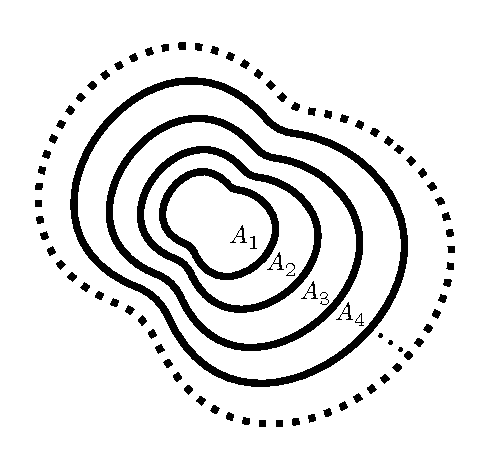
\includegraphics[trim=0cm 0cm 0cm 0cm, clip, scale=0.6]{images/misuracontinua1.pdf}
	\end{center}
	\item Per ogni successione di insiemi $A_n$ \textit{decrescente}, cioè tale che $A_{i+1}\subseteq A_i,\ \forall i\in\naturalset$, con $\mu(A_1)<+\infty$, si ha
		\begin{equation}
			\mu\left(\bigcap_{n\geq 1}A_n\right)=\lim_{n\to+\infty}\mu\left(A_n\right)
		\end{equation}
	e $\mu$ è detta \textbf{continua da sopra}\index{continuità!da sopra}.
	\begin{center}
		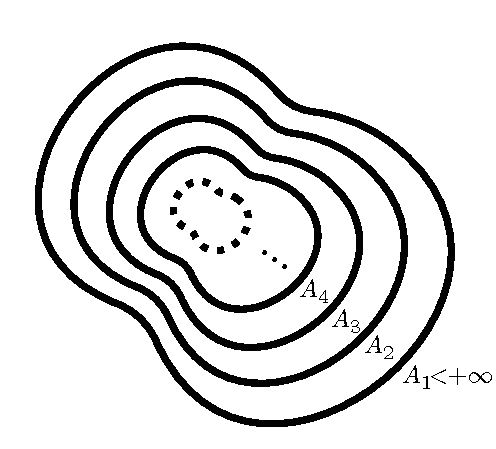
\includegraphics[trim=0cm 0cm 0cm 0cm, clip, scale=0.6]{images/misuracontinua2.pdf}
	\end{center}
	\end{itemize}
\end{property}
\begin{attention}
	Per la continuità da sopra è fondamentale l'ipotesi che $\mu\left(A_1\right)$ è finita.
\end{attention}
\begin{examplewt}[Controesempio alla continuità da sopra]
	Consideriamo la misura di Lebesgue unidimensionale $m_1$ e prendiamo la successione $A_n=\left[n,+\infty\right)$. Essa è decrescente in quanto
	\begin{equation*}
		A_{n+1}=\left[n+1,+\infty\right)\subsetneqq\left[n,+\infty\right)=A_n.
	\end{equation*}
	Si ha $m\left(A_n\right)=+\infty,\ \forall n$, e quindi in particolare
	\begin{equation*}
		\lim_{n\to+\infty}\mu\left(A_n\right)=+\infty
	\end{equation*}
	D'altro canto si ha
	\begin{equation*}
		\bigcap_{n\geq 1}A_n=\emptyset\implies\mu\left(\bigcap_{n\geq 1}A_n\right)=\mu\left(\emptyset\right)=0
	\end{equation*}
\end{examplewt}
\section{Famiglie di insiemi nella teoria della misura e relazioni tra di loro}\label{famigliediinsiemi}
Concludiamo questo capitolo alcune delle più comuni \textit{famiglie di insiemi} che si incontrano nello studio della teoria della misura.
\begin{center}
	\begin{tabular}{c|c|c}
		\textbf{Nome}                                                                            & \textbf{Notazione}                          & \textbf{Cardinalità}        \\ \hline
		Insieme delle parti                                                             & $\setpart{\realset}$               & $2^{\mathfrak{c}}$ \\ \hline
		\begin{tabular}[c]{@{}c@{}}Insiemi misurabili\\ (secondo Lebesgue)\end{tabular} & $\mathcal{L}\left(\realset\right)$ & $2^{\mathfrak{c}}$ \\ \hline
		Borelliani                                                                      & $\mathcal{B}\left(\realset\right)$ & $\mathfrak{c}$     \\ \hline
		\begin{tabular}[c]{@{}c@{}}Topologia\\ (famiglia degli aperti)\end{tabular}     & $\topo$                            & $\mathfrak{c}$    
	\end{tabular}
\end{center}
\begin{proposition}[Relazioni tra classi di insiemi]
	Valgono le seguenti inclusioni:
	\begin{equation}
		\topo\subsetneqq\mathcal{B}\left(\realset\right)\subsetneqq\mathcal{L}\left(\realset\right)\subsetneqq\setpart{\realset}
	\end{equation}
\end{proposition}
Mostreremo alcune di queste inclusioni in modo formale, mentre per altre daremo solo un'intuizione della dimostrazione.
\paragraph{Cardinalità dell'insieme delle parti dei reali}
Se $\abs{\realset}=\mathfrak{c}$ è la cardinalità del continuo, allora la cardinalità dell'\textit{insieme delle parti dei reali}\footnote{In ‘‘Brevi cenni di teoria degli insiemi'', a pag. \pageref{cardinalitàsetpart} è possibile trovare qualche dettaglio sulla cardinalità dell'insieme delle parti di un insieme e a pag. \pageref{cardinalitàsetpartreali} su quella dell'insieme delle parti dei reali.} è
\begin{equation}
	\abs{\setpart{\realset}}=2^{\mathfrak{c}}
\end{equation}
\paragraph{Cardinalità degli insiemi misurabili}
Per trovare quanti sono gli insiemi misurabili, consideriamo l'\textit{insieme di Cantor} $C$. Abbiamo visto\footnote{Si veda pag. \pageref{insiemecantor}.} che esso gode delle seguenti proprietà:
\begin{enumerate}
	\item Il numero di punti prima e dopo il processo iterativo per costruire $C$ rimane invariato, dunque $C$ è \textit{non numerabile} e ha la stessa cardinalità di $\left[0,1\right]$:
	\begin{equation*}
		\abs{C}=\abs{\left[0,1\right]}=\mathfrak{c}
	\end{equation*}
	\item $C$ è misurabile e $m_1\left(C\right)=0$.
\end{enumerate}
Dal punto 1 segue che l'insieme delle parti dell'insieme di Cantor ha cardinalità $\setpart{C}=2^{\mathfrak{c}}$, mentre dal punto 2 si può dedurre che ogni sottoinsieme di $C$ ha misura nulla ed è pertanto misurabile. Insiemisticamente parlando, le relazioni sono
\begin{equation*}
	\setpart{C}\subseteq \mathcal{L}\left(\realset\right)\subseteq\setpart{\realset}
\end{equation*}
Passando alle cardinalità:
\begin{equation*}
	2^{\mathfrak{c}}\underset{(1)}{=}{\abs{\setpart{C}}}\leq \abs{\mathcal{L}\left(\realset\right)}\leq\abs{\setpart{\realset}}=2^{\mathfrak{c}}\implies \abs{\mathcal{\realset}}=2^{\mathfrak{c}}
\end{equation*}
\paragraph{Inclusione stretta di {$\mathcal{L}\left(\realset\right)$} in {$\setpart{\realset}$}}
Il fatto che la cardinalità degli insiemi Lebesgue-misurabili in $\realset$ coincida con quella dell'insieme delle parti di $\realset$ non è sufficiente\footnote{Si veda ‘‘Brevi cenni di teoria degli insiemi'', pag. \pageref{cardinalitàugualenonimplicauguaglianzainsiemistica}.} per affermare che i due insiemi coincidano; costruiamo ora un sottoinsieme particolare di $\realset$ che risulta \textit{non misurabile}.
\begin{define}[Insieme di Vitali]\label{vitali}
	Considerata in $\realset$ la relazione di equivalenza
	\begin{equation}
		x\sim y\iff x-y\in\rationalset
	\end{equation}
	possiamo definire delle classi di equivalenza in $\nicefrac{\realset}{\sim}$:
	\begin{align*}
		\left[0\right]&=\left\{0,1,\frac{1}{2},-\frac{3}{4},\frac{123}{72},\ldots\right\}=\left\{x\in\realset\mid x\in\rationalset\right\}=\rationalset\\
		\left[\sqrt{2}\right]&=\left\{\sqrt{2},\sqrt{2}+\frac{1}{2},\sqrt{2}-1,\ldots\right\}=\left\{x\in\realset\mid x=\sqrt{2}+q,\ q\in\rationalset\right\}\\
		\left[\pi\right]&=\left\{\pi,\pi-\frac{3}{4},\pi+23,\ldots\right\}=\left\{x\in\realset\mid x=\pi+q,\ q\in\rationalset\right\}\\
		\vdots
	\end{align*}
	Scelto\footnote{Per poter fare questa operazione è necessario supporre l'\textit{Assioma di Scelta}.} un elemento che stia in $\left[0,1\right]$ da ogni classe di equivalenza, definisco l'\textbf{insieme di Vitali}\index{insieme!di Vitali} $V$ come unione di questi elementi.
\end{define}
Per costruzione $V\subseteq\left[0,1\right]$. Preso l'insieme \textit{numerabile} $\rationalset\cap\left[0,1\right]$, possiamo prendere una sua \textit{numerazione} $\left\{q_n\right\}$ e definire delle \textit{traslazioni} dell'insieme di Vitali $V$:
\begin{equation*}
	V_n=V+q_n\subseteq\left[-1,2\right]
\end{equation*}
\begin{lemming}[Lemma 1 di Vitali - gli insiemi di Vitali traslati sono 2 a 2 disgiunti]
	Dato l'insieme di Vitali $V$  e una enumerazione $\left\{q_n\right\}$  di $\rationalset\cap\left[0,1\right]$, allora $V_n\cap V_m=\emptyset,\ \forall n\neq m$.
\end{lemming}
\begin{demonstration}
	Consideriamo $x\in V_n\cap V_m$: questo implica che $x\in V_n$ e $x\in V_m$, ossia
	\begin{equation*}
		\begin{cases}
			x=y+q_n,\ y\in V,\ q_n\in\rationalset\cap\left[-1,1\right]\\
			x=z+q_m,\ z\in V,\ q_m\in\rationalset\cap\left[-1,1\right]
		\end{cases}
	\end{equation*}
	Pertanto,
	\begin{equation*}
		y+q_n=z+q_m\iff y-z=q_m-q_n\in\rationalset
	\end{equation*}
	Poichè $y$ e $z$ differiscono di un razionale, essi appartengono alla stessa classe di equivalenza in $\nicefrac{\realset}{\sim}$, ma dato che nella costruzione dell'insieme di VItali abbiamo preso\footnote{In virtù dell'\textit{Assioma di Scelta}.} uno e un solo elemento da tale classe, allora segue che $y=z$. È immediato verificare che $q_m=q_n$ e, essendo elementi numerazione, allora $n=m$. In altre parole, l'intersezione non è vuota solo se $V_n=V_m$.
\end{demonstration}
\begin{lemming}[Lemma 2 di Vitali - ogni numero reale in {$\left[0,1\right]$} appartiene ad un $V_n$ per un certo $n$:]
	Dato l'insieme di Vitali $V$ vale la seguente relazione:
	\begin{equation*}
		\left[0,1\right]\subseteq\bigcup_{n\in\naturalset}V_n
	\end{equation*}
\end{lemming}
\begin{demonstration}
	Sia $x\in\left[0,1\right]$. Poiché la relazione $\sim$ forma una partizione di $\realset$, deve esistere $y$ tale che $x-y=q\in\rationalset$; riscrivendo tale relazione si ha $x=y+q$, ossia $x=y+q_n$ per un certo $n$.
\end{demonstration}
Possiamo osservare alcune proprietà sulla base dei due lemmi appena mostrati:
\begin{itemize}
	\item \textbf{Conseguenze del lemma 1:}
	\begin{equation*}
		m\left(\bigcup_{n\in\naturalset}V_n\right)=\sum_{n\in\naturalset}m\left(V_n\right)=\sum_{n\in\naturalset}m\left(V\right)=\begin{cases}
			\begin{array}{ll}
				0&\text{se }m\left(V\right)=0\\
				+\infty&\text{se }m\left(V\right)>0
			\end{array}
		\end{cases}
	\end{equation*}
	\item \textbf{Conseguenze del lemma 2:}
	\begin{equation*}
		1=m\left(\left[0,1\right]\right)\leq m\left(\bigcup_{n\in\naturalset}V_n\right)\leq m\left(\left[-1,2\right]\right)=3
	\end{equation*}
\end{itemize}
In altre parole, si deduce che
\begin{equation*}
	1\leq \sum_{n\in\naturalset}m\left(V\right)\leq 3
\end{equation*}
ma poiché la somma di infinite copie di $m\left(V\right)$ o è $0$ o è $+\infty$ per la conseguenza del lemma 1, in nessuno dei due casi la somma sta in $\left[1,3\right]$. Pertanto, $V$ \textit{non} è misurabile, in quanto non possiamo associargli un valore $m\left(V\right)$.
\paragraph{Cardinalità dei Borelliani e inclusione stretta di {$\mathcal{B}\left(\realset\right)$} in {$\mathcal{L}\left(\realset\right)$}}
Per \textit{induzione transfinita} si dimostra che i Borelliani hanno la cardinalità del continuo.
\begin{equation}
	\abs{\mathcal{B}\left(\realset\right)}=\abs{\realset}=\mathfrak{c}
\end{equation}
Pertanto, l'inclusione $\mathcal{B}\left(\realset\right)\subsetneqq \mathcal{L}\left(\realset\right)$ è stretta.
\begin{digression}
	L'Assioma della Scelta \textit{non} è necessario per dimostrare l'inclusione stretta di $\mathcal{B}\left(\realset\right)$ in $\mathcal{L}\left(\realset\right)$. Infatti, si può costruire un insieme misurabile \textit{non} Borelliano senza farne uso.
\end{digression}